\documentclass{article}
\usepackage{background}
\usepackage[utf8]{inputenc}
\usepackage{geometry}
\usepackage[bottom]{footmisc}
 \geometry{
 a4paper,
 total={170mm,257mm},
 left=20mm,
 top=10mm,
 }

\title{2020.08.19 Class Learning Plan  MAD 5274_1}
\author{Instructor: Peter Sigurdson }
\date{Wednesday, August 19, 2020 Summer}

\begin{document}
\backgroundsetup{scale = 1, angle = 0, opacity = 0.1,
  contents = {
\includegraphics[width = \paperwidth,
  height = \paperheight, keepaspectratio] {111.png}}}
\maketitle

\section * {Key Topics:}
% attendance quiz: https://www.classmarker.com/online-test/start/?quiz=vvh5f3d12c8a45b4
\section{Milestone 2 handin LINK}
\url{https://t2m.io/MAD5274S1_MILESTONE2_HANDIN}

\subsection{Testing the MOBILE APP}
\url{https://t2m.io/MobileAppsTestingLabFlow1}

\subsection{Review Yesterday's Topics}

\subsection{Constructing Use Cases}
\subsection{The Traceability Matrix}
\subsection{Project Management Considerations in developing the Mobile App}

\item Project Management - Comparing Traditional Project Management with the special requirements of Software Development
\item Traceability Matrix and building test cases.
\item Relating use cases to the Project Management Plan Work Breakdown Structure.
\item Agile and Scrum Project Leadership Skills (Text Reference)

\section{The most important document in Project Management:}

CREATE WBS Create WBS is the process of subdividing project deliverables and project work into smaller, more manageable components. The key benefit of this process is that it provides a framework of what has to be delivered. This process is performed once or at predefined points in the project. The inputs, tools and techniques, and outputs of this process are depicted in Figure 5-10. Figure 5-11 depicts the data flow diagram of the process.\\

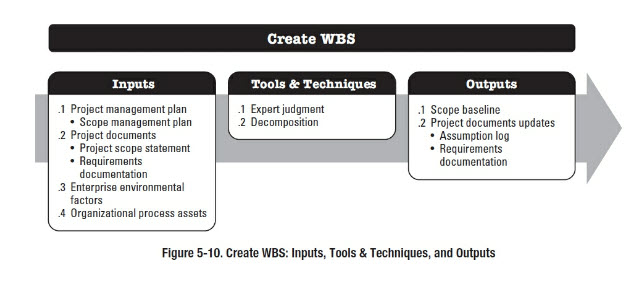
\includegraphics[]{createWBS.jpg}

5.4.2 CREATE WBS: TOOLS AND TECHNIQUES \\

5.4.2.1 EXPERT JUDGMENT Described in Section 4.1.2.1. \\

Expertise should be considered from individuals or groups with knowledge of or experience with similar projects. 

\\

5.4.2.2 DECOMPOSITION Decomposition is a technique used for dividing and subdividing the project scope and project deliverables into smaller, more manageable parts. The work package is the work defined at the lowest level of the WBS for which cost and duration can be estimated and managed. 
\\

The level of decomposition is often guided by the degree of control needed to effectively manage the project. The level of detail for work packages will vary with the size and complexity of the project. Decomposition of the total project work into work packages generally involves the following activities: Identifying and analyzing the deliverables and related work, Structuring and organizing the WBS, Decomposing the upper WBS levels into lower-level detailed components, Developing and assigning identification codes to the WBS components, and Verifying that the degree of decomposition of the deliverables is appropriate. A portion of a WBS with some branches of the WBS decomposed down through the work package level is shown in Figure 5-12. 
\newline



Project Management Institute. A Guide to the Project Management Body of Knowledge (PMBOK(R) Guide–Sixth Edition / Agile Practice Guide Bundle (Pmbok Guide) (p. 158). Project Management Institute. Kindle Edition. 

\footnote{Note: The Latex Code for this Document is available in my GitHub Repository at 
    Computational Knowledge. I welcome and encourage you to use my Latex to develop your 
    own study notes for this course.}
 
\end{document}